\chapter{Material adicional}
\label{chap:adicional}

\section{Figuras adicionais}
\label{sec:figuras_adicionales}

\subsection{Figuras experimentos de resolución}
\label{subsec:figuras_experimentos_resolucion}

\begin{table}[h]
    \centering
    \begin{minipage}[t]{0.45\linewidth}
        \centering
        \scriptsize
        \setlength{\tabcolsep}{25pt}
        \begin{tabular}{|c|c|}
        \hline
        Resolution & Mean Distance \\ \hline
        100 & 254.22 \\ \hline
        250 & 251.29 \\ \hline
        750 & 250.62 \\ \hline
        1250 & 250.59 \\ \hline
        1708 & 249.72 \\ \hline
        \end{tabular}
        \caption{Distancias medias para o dataset FIRE ca función de activación Relu}
        \label{tab:mlp_mean_distances_fire}
    \end{minipage}
    \hfill
    \begin{minipage}[t]{0.45\linewidth}
        \centering
        \scriptsize
        \setlength{\tabcolsep}{25pt}
        \begin{tabular}{|c|c|}
        \hline
        Resolution & Mean Distance \\ \hline
        100 & 266.43 \\ \hline
        250 & 263.85 \\ \hline
        750 & 263.19 \\ \hline
        1250 & 258.56 \\ \hline
        1708 & 258.06 \\ \hline
        \end{tabular}
        \caption{Distancias medias para o dataset FIRE ca función de activación SIREN}
        \label{tab:siren_mean_distances_fire}
    \end{minipage}
\end{table}

\begin{table}[h]
    \centering
    \begin{minipage}[t]{0.45\linewidth}
        \centering
        \scriptsize
        \setlength{\tabcolsep}{25pt}
        \begin{tabular}{|c|c|}
        \hline
        Resolution & Mean Distance \\ \hline
        100 & 37.29 \\ \hline
        250 & 36.18 \\ \hline
        750 & 36.01 \\ \hline
        1250 & 35.03 \\ \hline
        1708 & 35.04 \\ \hline
        \end{tabular}
        \caption{Distancias medias para o dataset RFMID ca función de activación Relu}
        \label{tab:mlp_mean_distances_rfmid}
    \end{minipage}
    \hfill
    \begin{minipage}[t]{0.45\linewidth}
        \centering
        \scriptsize
        \setlength{\tabcolsep}{25pt}
        \begin{tabular}{|c|c|}
        \hline
        Resolution & Mean Distance \\ \hline
        100 & 68.12 \\ \hline
        250 & 73.42 \\ \hline
        750 & 77.55 \\ \hline
        1250 & 67.33 \\ \hline
        1708 & 67.31 \\ \hline
        \end{tabular}
        \caption{Distancias medias para o dataset RMIFD ca función de activación SIREN}
        \label{tab:siren_mean_distances_rfmid}
    \end{minipage}
\end{table}


\subsection{Figuras experimentos de regularización}
\label{subsec:figuras_experimentos_regularizacion}

\begin{figure}[ht]
    \centering
    \begin{subfigure}[b]{0.4\textwidth}
        \centering
        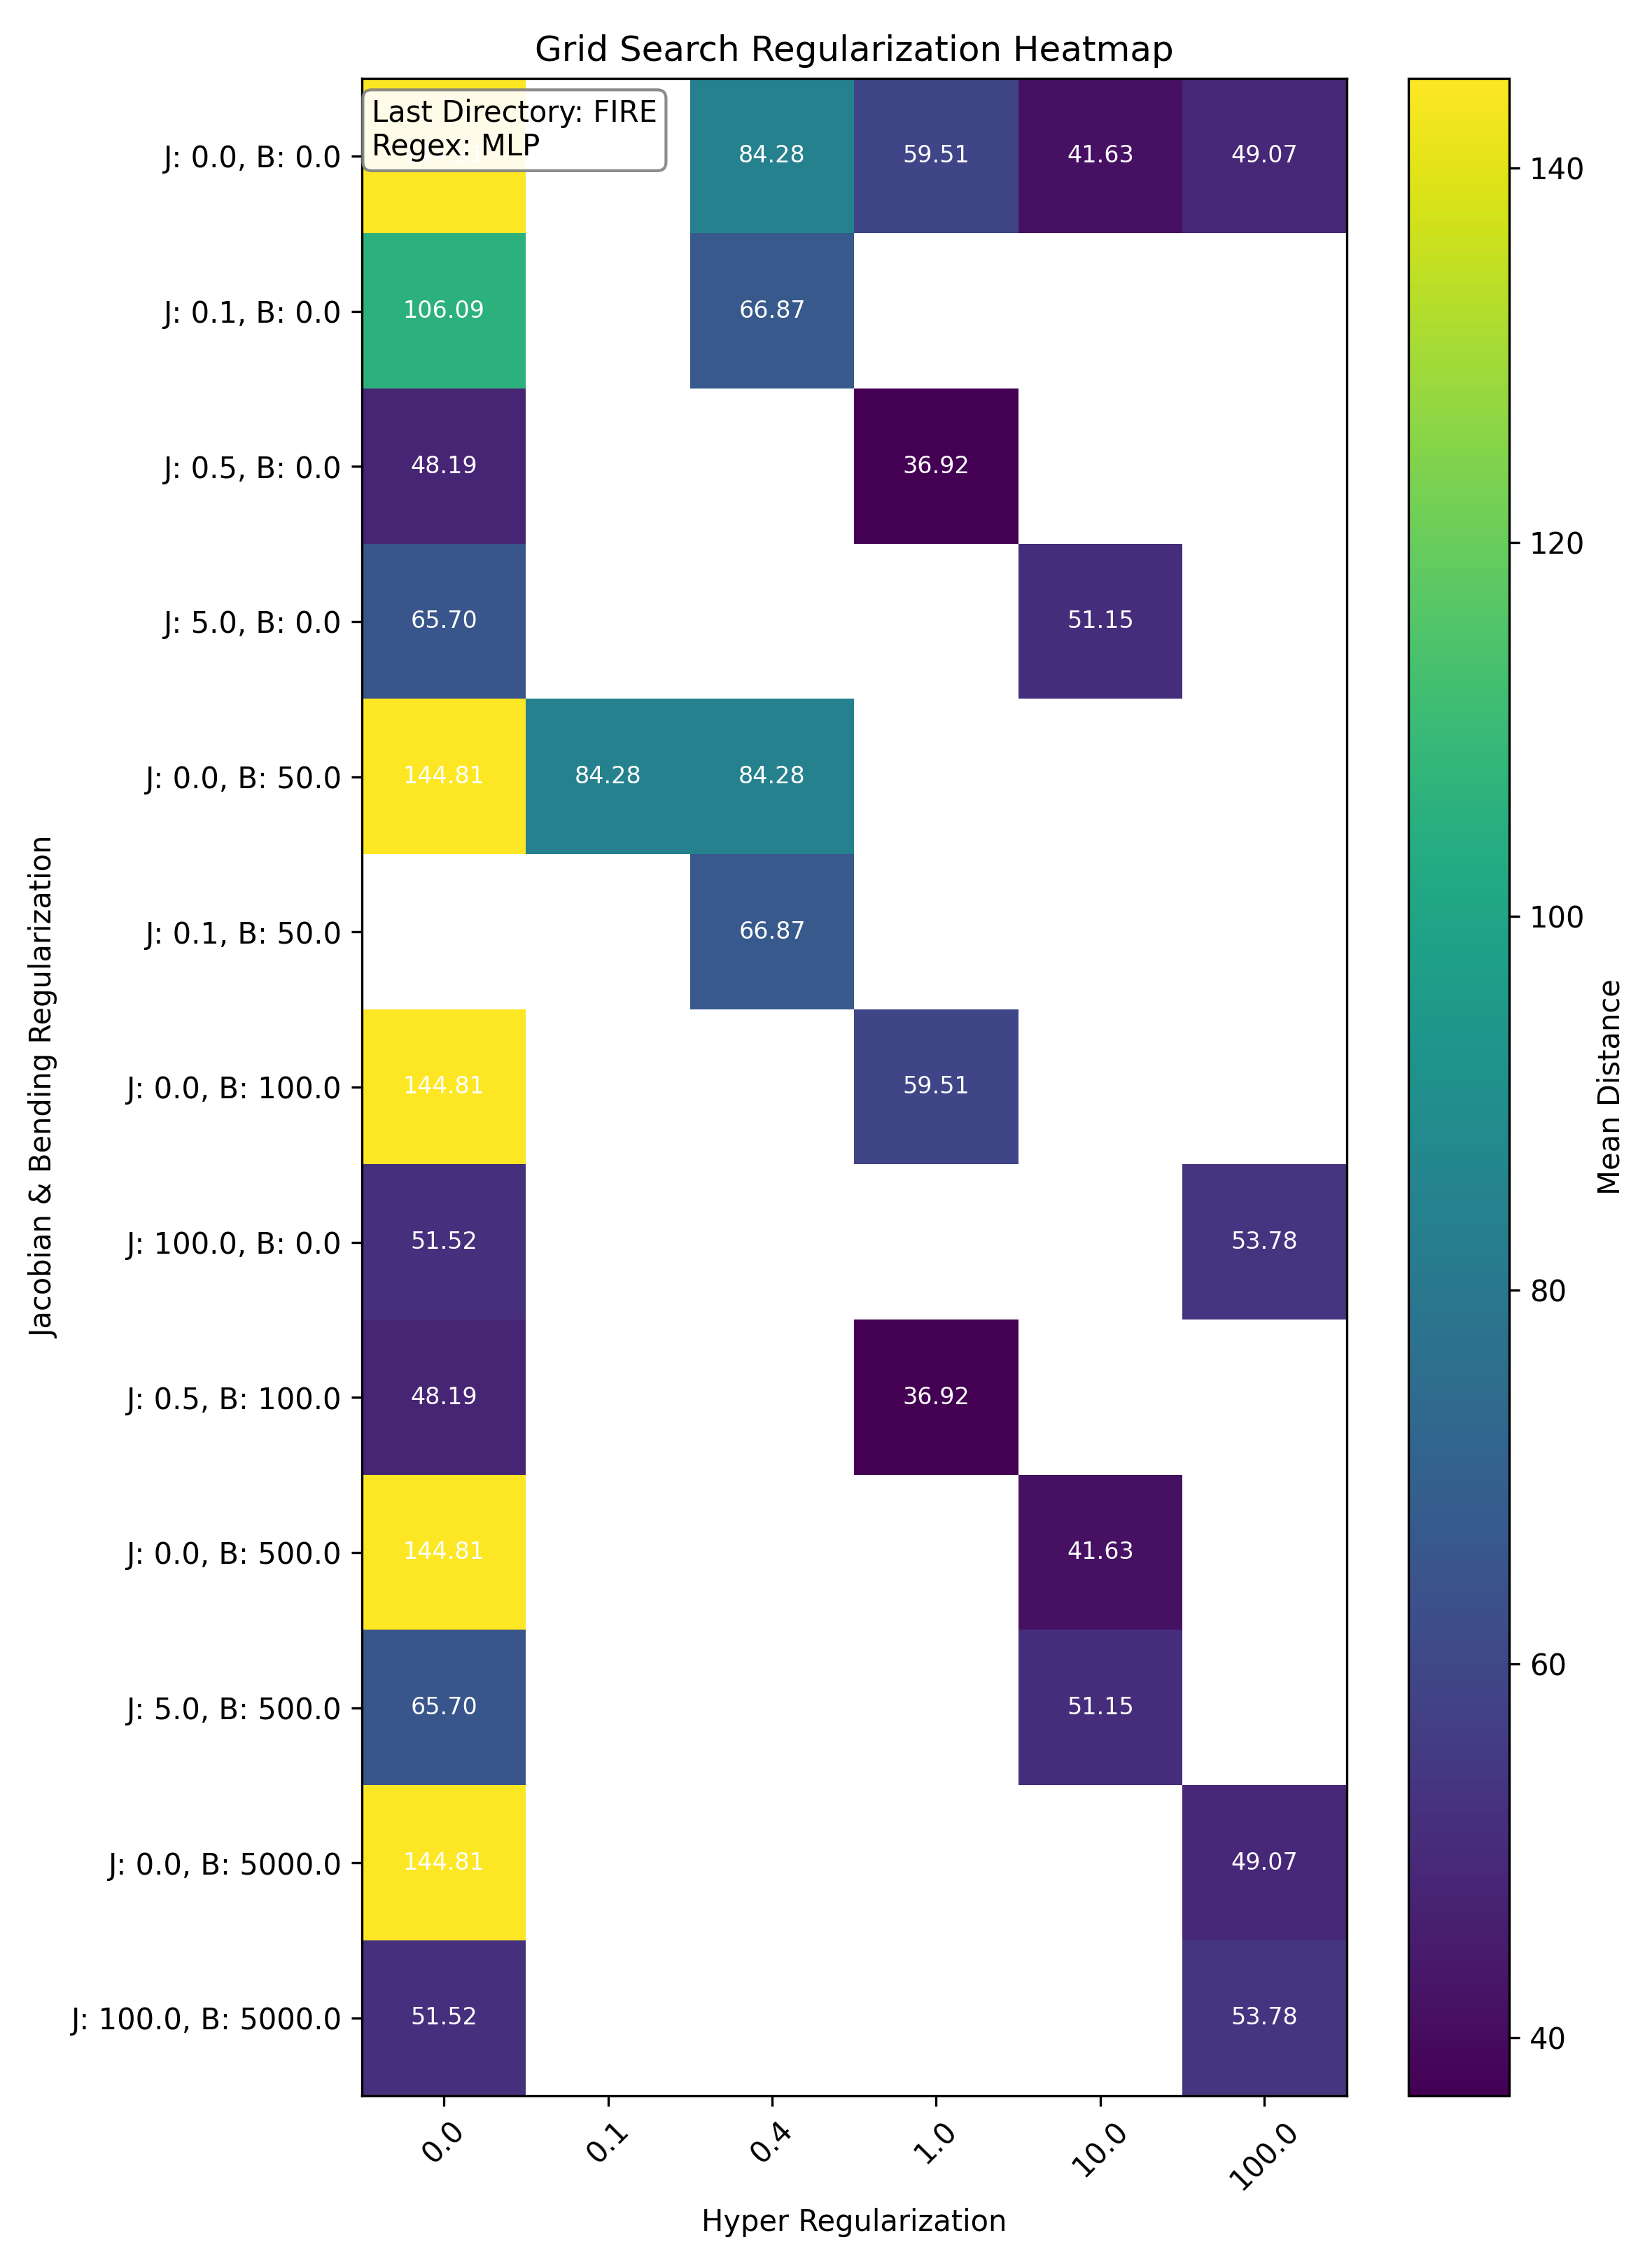
\includegraphics[width=\textwidth]{imaxes/grid_search_single_heatmap_FIRE_MLP.png}
        \caption{FIRE - Relu}
        \label{fig:gs_single_FIRE_MLP}
    \end{subfigure}\hfill
    \begin{subfigure}[b]{0.4\textwidth}
        \centering
        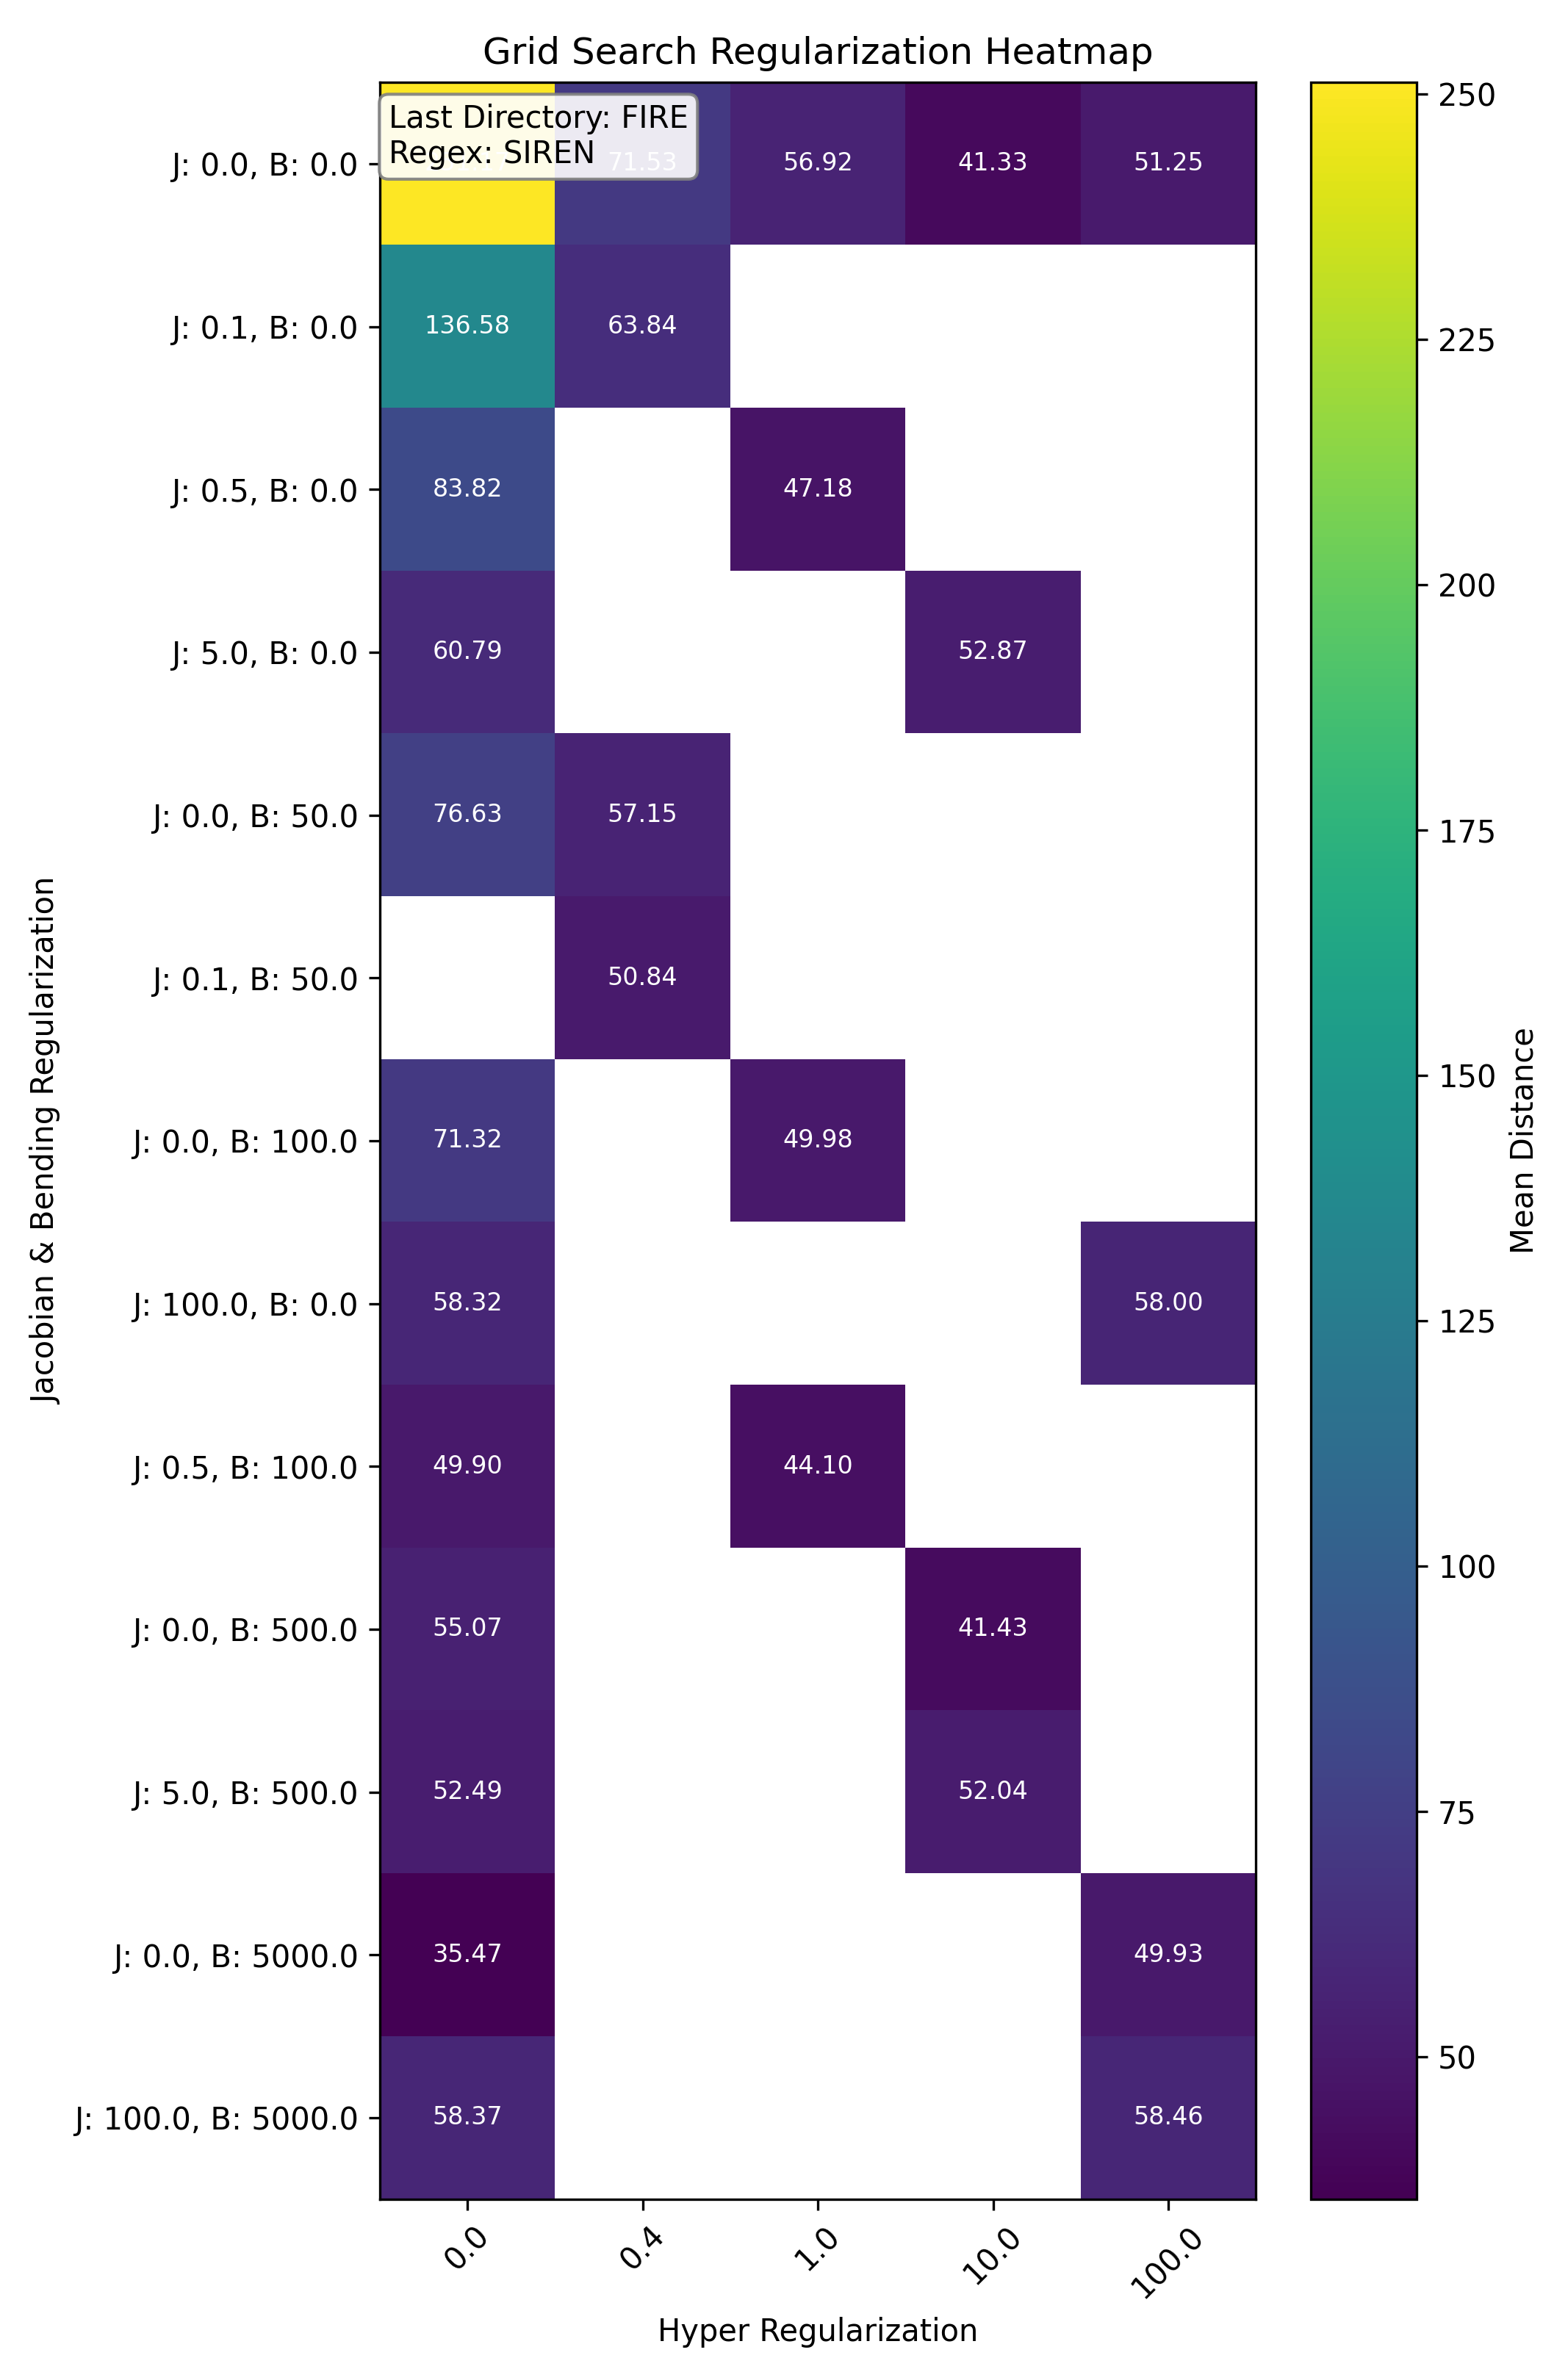
\includegraphics[width=\textwidth]{imaxes/grid_search_single_heatmap_FIRE_SIREN.png}
        \caption{FIRE - SIREN}
        \label{fig:gs_single_FIRE_SIREN}
    \end{subfigure}
    
    \vskip0\baselineskip
    
    \begin{subfigure}[b]{0.4\textwidth}
        \centering
        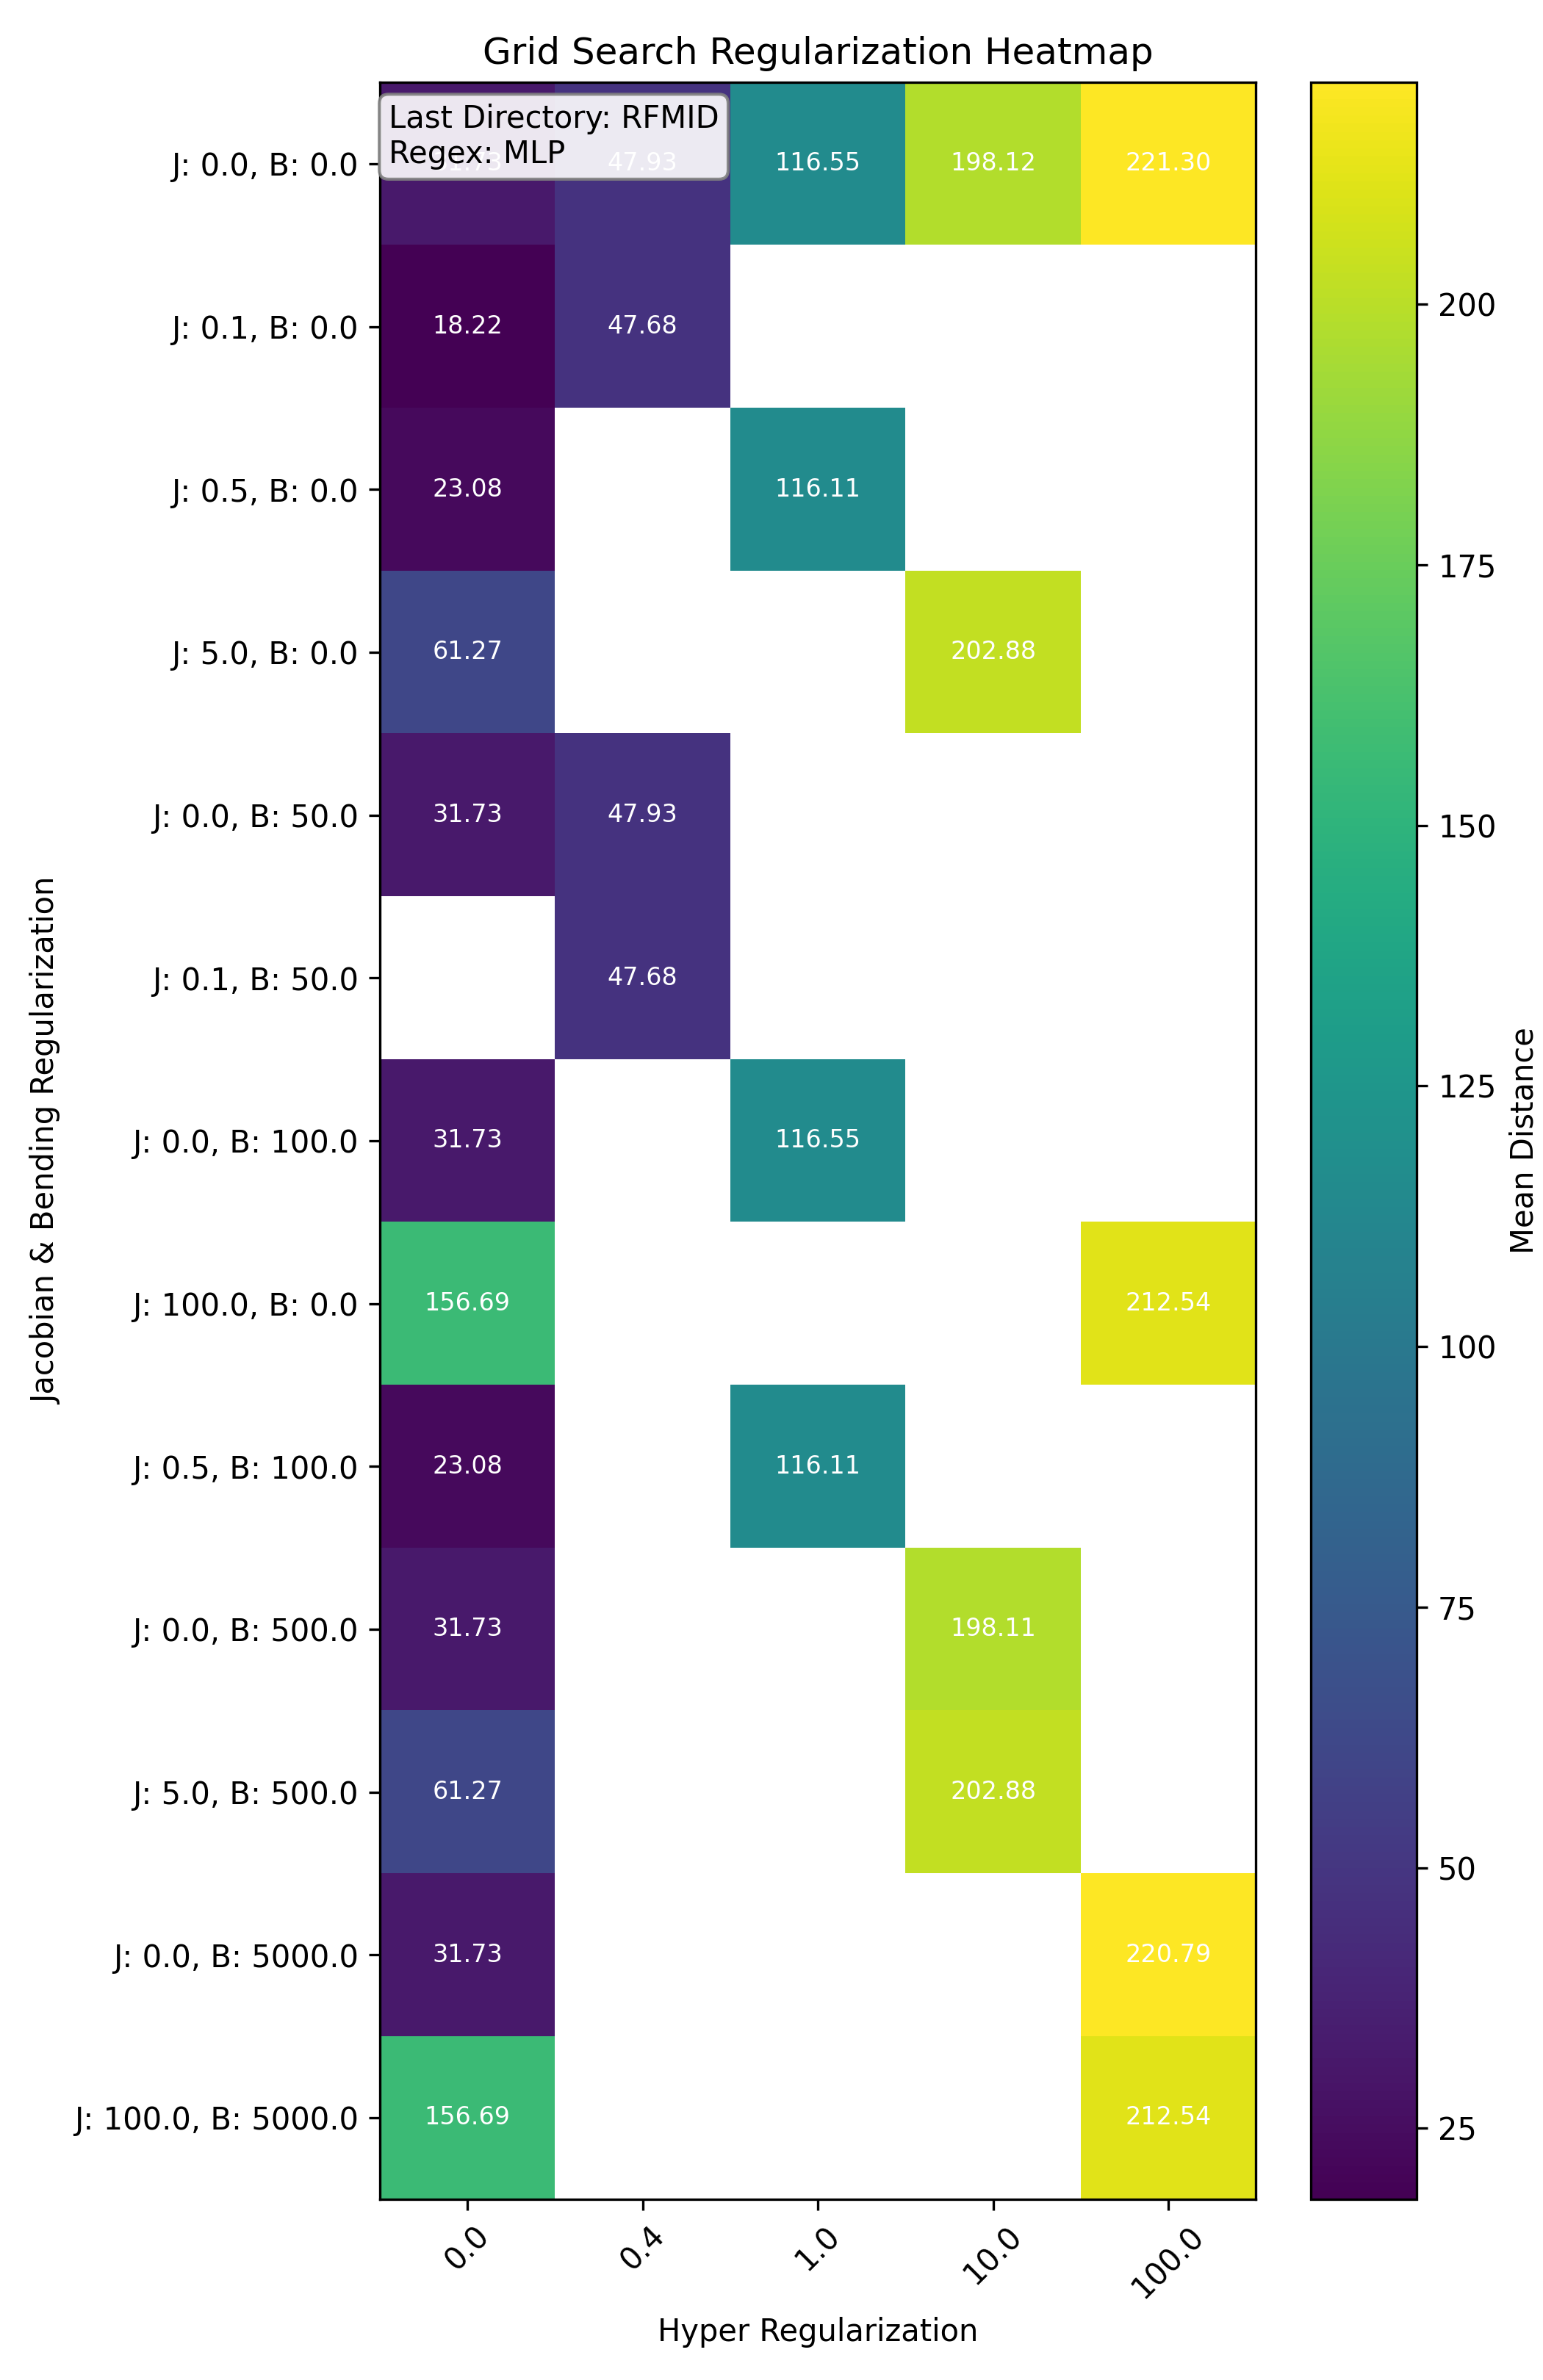
\includegraphics[width=\textwidth]{imaxes/grid_search_single_heatmap_RFMID_MLP.png}
        \caption{RFMID - Relu}
        \label{fig:gs_single_RFMID_MLP}
    \end{subfigure}\hfill
    \begin{subfigure}[b]{0.4\textwidth}
        \centering
        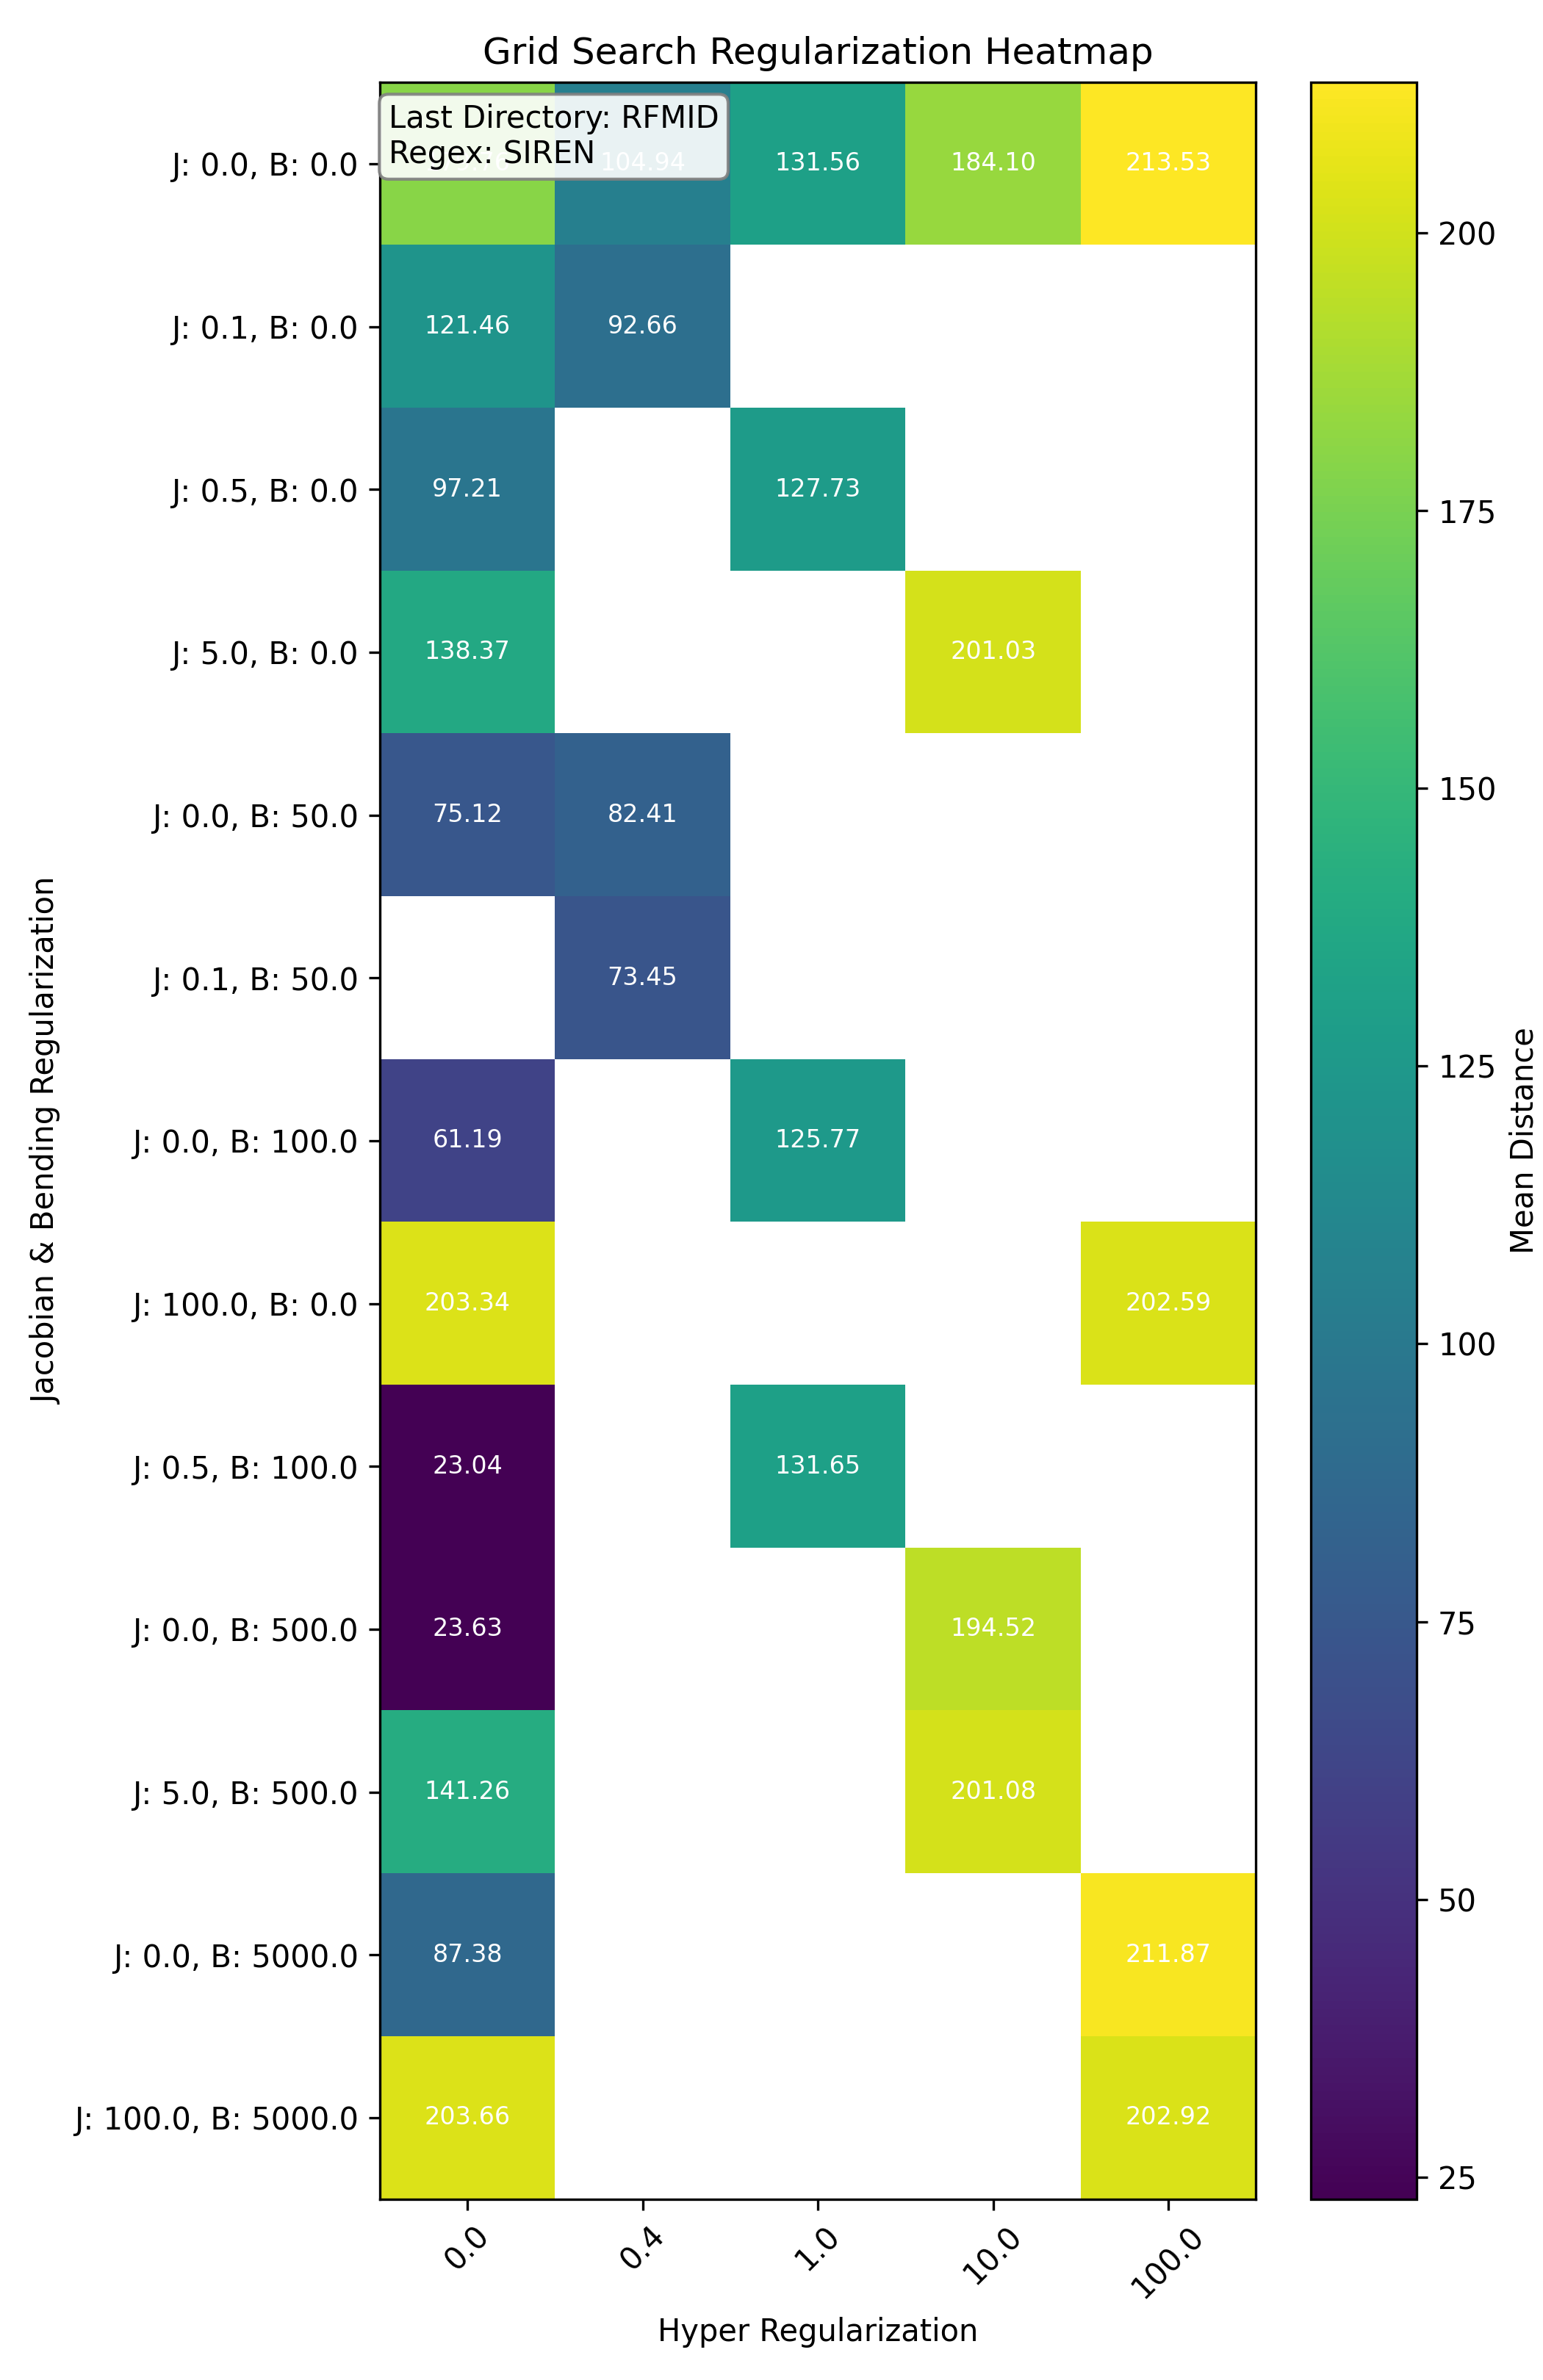
\includegraphics[width=\textwidth]{imaxes/grid_search_single_heatmap_RFMID_SIREN.png}
        \caption{RFMID - SIREN}
        \label{fig:gs_single_RFMID_SIREN}
    \end{subfigure}
    
    \caption{Mapa de calor cos resultados de diferentes combinacións de termos de regularización e funcións de activación sobre os datasets FIRE e RFMID}
    \label{fig:gs_single_heatmaps}
\end{figure}